\documentclass[xcolor=dvipsnames, 10pt]{beamer}
\usepackage[utf8]{inputenc}
\usepackage{enumitem,xcolor}
% \usetheme{CambridgeUS}
\usepackage{libertine}
\usepackage{enumerate}
\usepackage{booktabs}

\usepackage{MnSymbol,wasysym}
\usepackage{ragged2e}
\usepackage{threeparttable}
\justifying

\definecolor{blue}{HTML}{1a296b}
% \definecolor{lightblue}{HTML}{009bbd}
\definecolor{lightblue}{RGB}{86,76,169}
\definecolor{grey}{HTML}{C3C5C2}
\definecolor{white}{HTML}{FDFEFE}
\definecolor{darkred}{rgb}{0.8,0,0}
\definecolor{myGrey}{rgb}{.7,.7,.7}
\usepackage{color}
\definecolor{twi}{RGB}{86,76,169}
\definecolor{TWI}{RGB}{86,76,169}
\newcommand{\old}[1]{{\color{myGrey} #1\color{black}}}
\newcommand{\orange}[1]{{\color{orange} #1\color{black}}}
\newcommand{\iw}[1]{{\color{blue} #1\color{black}}}
\newcommand{\twi}[1]{{\color{TWI} #1\color{black}}}


\setbeamercolor{normal text}{fg=black,bg=white}
\setbeamercolor{alerted text}{fg=blue}
\setbeamercolor{example text}{fg=black}
\setbeamercolor{title}{fg=TWI}
\setbeamercolor{frametitle}{fg=TWI}
\setbeamercolor{structure}{fg=TWI}
% \setbeamercovered{dynamic}
% \setbeamercovered{transparent=5}
\setbeamercovered{%
	still covered={\opaqueness<1>{4}\opaqueness<2>{2}\opaqueness<3>{1}\opaqueness<4->{1}},
	again covered={\opaqueness<1->{50}}}
\setbeamertemplate{navigation symbols}{}

\setbeamercolor{palette primary}{fg=white, bg=blue}
\setbeamercolor{palette secondary}{fg=white, bg=blue}
\setbeamercolor{palette tertiary}{fg=white, bg=lightblue}

\setbeamercolor{button}{bg=blue,fg=white}

\setlist[itemize,1]{label=$\color{lightblue}\blacktriangleright$}
\setlist[itemize,2]{label=\boldmath$\color{lightblue}\cdot$}

\usepackage{caption}
% \usepackage[labelfont={color=blue}]{caption}
% \makeatletter
% \setbeamertemplate{title page}[default][colsep=-4bp,rounded=true]
% \setbeamertemplate{footline}{%
	%     \leavevmode%
	%     \hbox{%
		%         \begin{beamercolorbox}[wd=.2\paperwidth,ht=2.25ex,dp=1ex,center]{author in head/foot}%
			%             \usebeamerfont{author in head/foot}\insertshortauthor\expandafter\beamer@ifempty\expandafter{\beamer@shortinstitute}{}{~~(\insertshortinstitute)}
			%         \end{beamercolorbox}%
		%         \begin{beamercolorbox}[wd=.6\paperwidth,ht=2.25ex,dp=1ex,center]{title in head/foot}%
			%             \usebeamerfont{title in head/foot}\insertshorttitle
			%         \end{beamercolorbox}%
		%         \begin{beamercolorbox}[wd=.2\paperwidth,ht=2.25ex,dp=1ex,right]{date in head/foot}%
			%             \usebeamerfont{date in head/foot}\insertshortdate{}\hspace*{2em}
			%             \insertframenumber{} / \inserttotalframenumber\hspace*{2ex}
			%         \end{beamercolorbox}}%
	%         \vskip0pt%
	%     }
% \makeatother

\setbeamertemplate{headline}{}
\setbeamertemplate{footline}{}

\title[Title]{\textbf{When personalization deters delegation to
		algorithms:\\ Evidence from a preregistered
		experiment}}
\author[I.Wolff\hspace{1.3cm}]{Irenaeus Wolff\\\vspace{.2cm}\footnotesize Thurgau Institute of Economics (TWI), \\University of Konstanz}
\date[Wolff @ AI WS 2026]{AI Workshop (Berlin), 23$^{\text{rd}}$ June, 2026}

% \logo{\includegraphics[scale = .17]{TWI_logo_for_presentations_TITLE_bg.pdf}\vspace{220pt} \hspace{-.15cm}}


\begin{document}
	\logo{
\includegraphics[scale = .37]{logo_twi_cmyk.pdf}\vspace{220pt} \hspace{-.15cm}}
	% THIS IS THE TITLEFRAME
	\begin{frame}
		\vspace{4.0cm}
		{\LARGE \twi{When personalization deters delegation to algorithms: Experimental evidence}}%\vspace{.2cm}}\\ 
	\\
	\vspace{.5cm}
	{\large Lara Suraci \& Irenaeus Wolff}\vspace{.1cm}\\
	{\small  --- 23$^\text{rd}$ June, 2026, Symposium on `AI and the Future of Work', Berlin ---}
\end{frame}

\logo{}


%This redefines the background for the regular slides(i.e. the smaller logo in the top-right corner)
\logo{
\includegraphics[scale = 0.25]{logo_twi_cmyk.pdf}\vspace{225pt} \hspace{-.12cm}}


%
% \author[Lara Suraci]{Lara Suraci \newline with Robin Cubitt, Chris Starmer and Irenaeus Wolff}
% \date[]{19 April 2023}
%
% \AtBeginSection[]
% {
	%   \begin{frame}
		%     \frametitle{Table of Contents}
		%     \tableofcontents[currentsection]
		%   \end{frame}
	% }
%
% \begin{document}
	% \setbeamertemplate{section in toc}[sections numbered]
	%
	% 	\begin{frame}
		% 	\titlepage
		% \centering
		% \includegraphics[scale=0.33]{notts_logo2.png}
		% 	\end{frame}
	
	
	\frame{\frametitle{Background}
		\begin{itemize}
			\item Huge \& unconnected literature on algorithm/automation/AI/... reliance %($\rightarrow$ review by Chugunova \& Sele, 2022)
			\item Most of the literature: setups with clearly identifiable mistakes
			\item But in many real-life settings, preferences determine what is a mistake
			\item E.g., robo-advisors: maximal payoff \textit{vs} best fit to risk-parameters
			%   \item[\twi{$\rightarrow$}]<2-> Our (first) research question!
			%   \item[\twi{No. 2:}]<2-> What are the consequences of feedback under either variant?
			%   \item[\twi{$\rightarrow$}]<2->  overweighting of algorithmic errors (Madhavan \& Wiegmann, 2007; Dietvorst et al. 2015; Hoff \& Bashir, 2015)
		\end{itemize}
	}
	
	
	\frame{\frametitle{Research Question}
		\begin{itemize}
			\item Does algorithm reliance differ for \textcolor{lightblue}{\textbf{objective optimization  \textit{vs.} preference-based personalisation}} in a preferential-choice environment?%\vspace{.2cm}
			\begin{itemize}
				\item[(i)] ...at first contact?
				\item[(ii)] ...overall?
			\end{itemize}
		\end{itemize}
	}
	
	\begin{frame}
		\frametitle{Objective vs Personalised Algorithms}%\vspace{1.5cm}}
	\begin{itemize}
		\setlength\itemsep{1em}
		%\item in BB, I will call it normative but just explain that this can be discussed “only a label, not an assertion that it is rational to be risk-averse” (same for PT, attempt to capture parameters, no one is asserting that PT is perfect as a model)
		\item What do we mean by \textcolor{lightblue}{\textbf{objective optimization}}?%\\\smallskip
		\begin{itemize}
			\item an algorithm that chooses some ‘objectively ideal’ option independently of a subject’s preferences (here: \textcolor{lightblue}{\textbf{highest EV}})\vspace{-.2cm}
		\end{itemize}
		\item What do we mean by \textcolor{lightblue}{\textbf{personalised}}?%\\\smallskip
		\begin{itemize}
			\item an algorithm that measures a subject’s preferences and chooses accordingly (here: \textcolor{lightblue}{\textbf{implementation of revealed preferences}})\vspace{-.2cm}
		\end{itemize}
	\end{itemize}
\end{frame}


\begin{frame}
	\frametitle{Objective vs Personalised Algorithms\vspace{.3cm}}
	\begin{itemize}
		\setlength\itemsep{1em}
		%\item in BB, I will call it normative but just explain that this can be discussed “only a label, not an assertion that it is rational to be risk-averse” (same for PT, attempt to capture parameters, no one is asserting that PT is perfect as a model)
		\item What do we mean by \textcolor{lightblue}{\textbf{objective optimization}}?%\\\smallskip
		\begin{itemize}
			\item an algorithm that chooses some ‘objectively ideal’ option independently of a subject’s preferences (here: \textcolor{lightblue}{\textbf{highest EV}})\vspace{-.2cm}
		\end{itemize}
		\item What do we mean by \textcolor{lightblue}{\textbf{personalised}}?%\\\smallskip
		\begin{itemize}
			\item an algorithm that measures a subject’s preferences and chooses accordingly (here: \textcolor{lightblue}{\textbf{implementation of revealed preferences}})\vspace{-.2cm}
		\end{itemize}
		\item In the experiment, we describe both algorithms in intuitive terms:\\\medskip \textcolor{lightblue}{\textbf{EV}}: \textit{‘The algorithm works out how much each option would yield on average and selects the option for which this is highest.’}\\\smallskip
		\textcolor{lightblue}{\textbf{Prefs}}: \textit{‘The algorithm analyses your choices from Part 1 and selects the best option for you in light of your Part-1 choices.’}
	\end{itemize}
\end{frame}

\frame{\frametitle{Relevance?}
	Well-known (Swiss) robo-advisors(' marketing strategies)
	\begin{itemize}
		\item ``We rely on a low-cost, passive investment strategy and have selected a total of 9 equity, bond and real estate ETFs from over 1,500 ETFs (exchange-traded funds) and put them together in such a way that they \twi{achieve an optimal risk/return ratio}.'' (findependent.ch; for GER, see e.g., whitebox.eu)
		\item ``Chat with Selma: Selma \twi{looks at your financial life and learns how you should structure your finances}. Get your plan: Selma \twi{creates a personalized investment plan that fits your life}. Sit back and relax! Selma takes care of your money from now on and does all the buying and selling for you.'' (selma.com; for GER, see e.g., quirion.de)
	\end{itemize}
}

\begin{frame}
	\frametitle{Experimental Design}%\vspace{2.5cm}}
\begin{itemize}
	\setlength\itemsep{1em}
	\item[\textcolor{lightblue}{\textbf{Part 1}}] \textcolor{lightblue}{-- } Elicitation of preferences
	\begin{itemize}
		\item only two, `well-presented' lotteries, unlimited time
		\item ``hypothetical, but the choices may be meaningful for Part 2''
	\end{itemize}
	\item[\textcolor{lightblue}{\textbf{Part 2}}] \textcolor{lightblue}{-- } Lottery Selection Task
	\begin{itemize}
		\item could stand for an investment task
		\item complexity (number of options, outcomes under different SOTW)
		\item time pressure (think: relative to the number of options)
        \item each Part-2 task built from 2 {anchor options} ($\rightarrow$ Part 1) + 6 {decoys}
		%      \item robo-advisors: opaque, `personalisable', supposedly `optimal'
	\end{itemize}
	
\end{itemize}
\end{frame}

\frame{\frametitle{Tasks}
\begin{figure}
	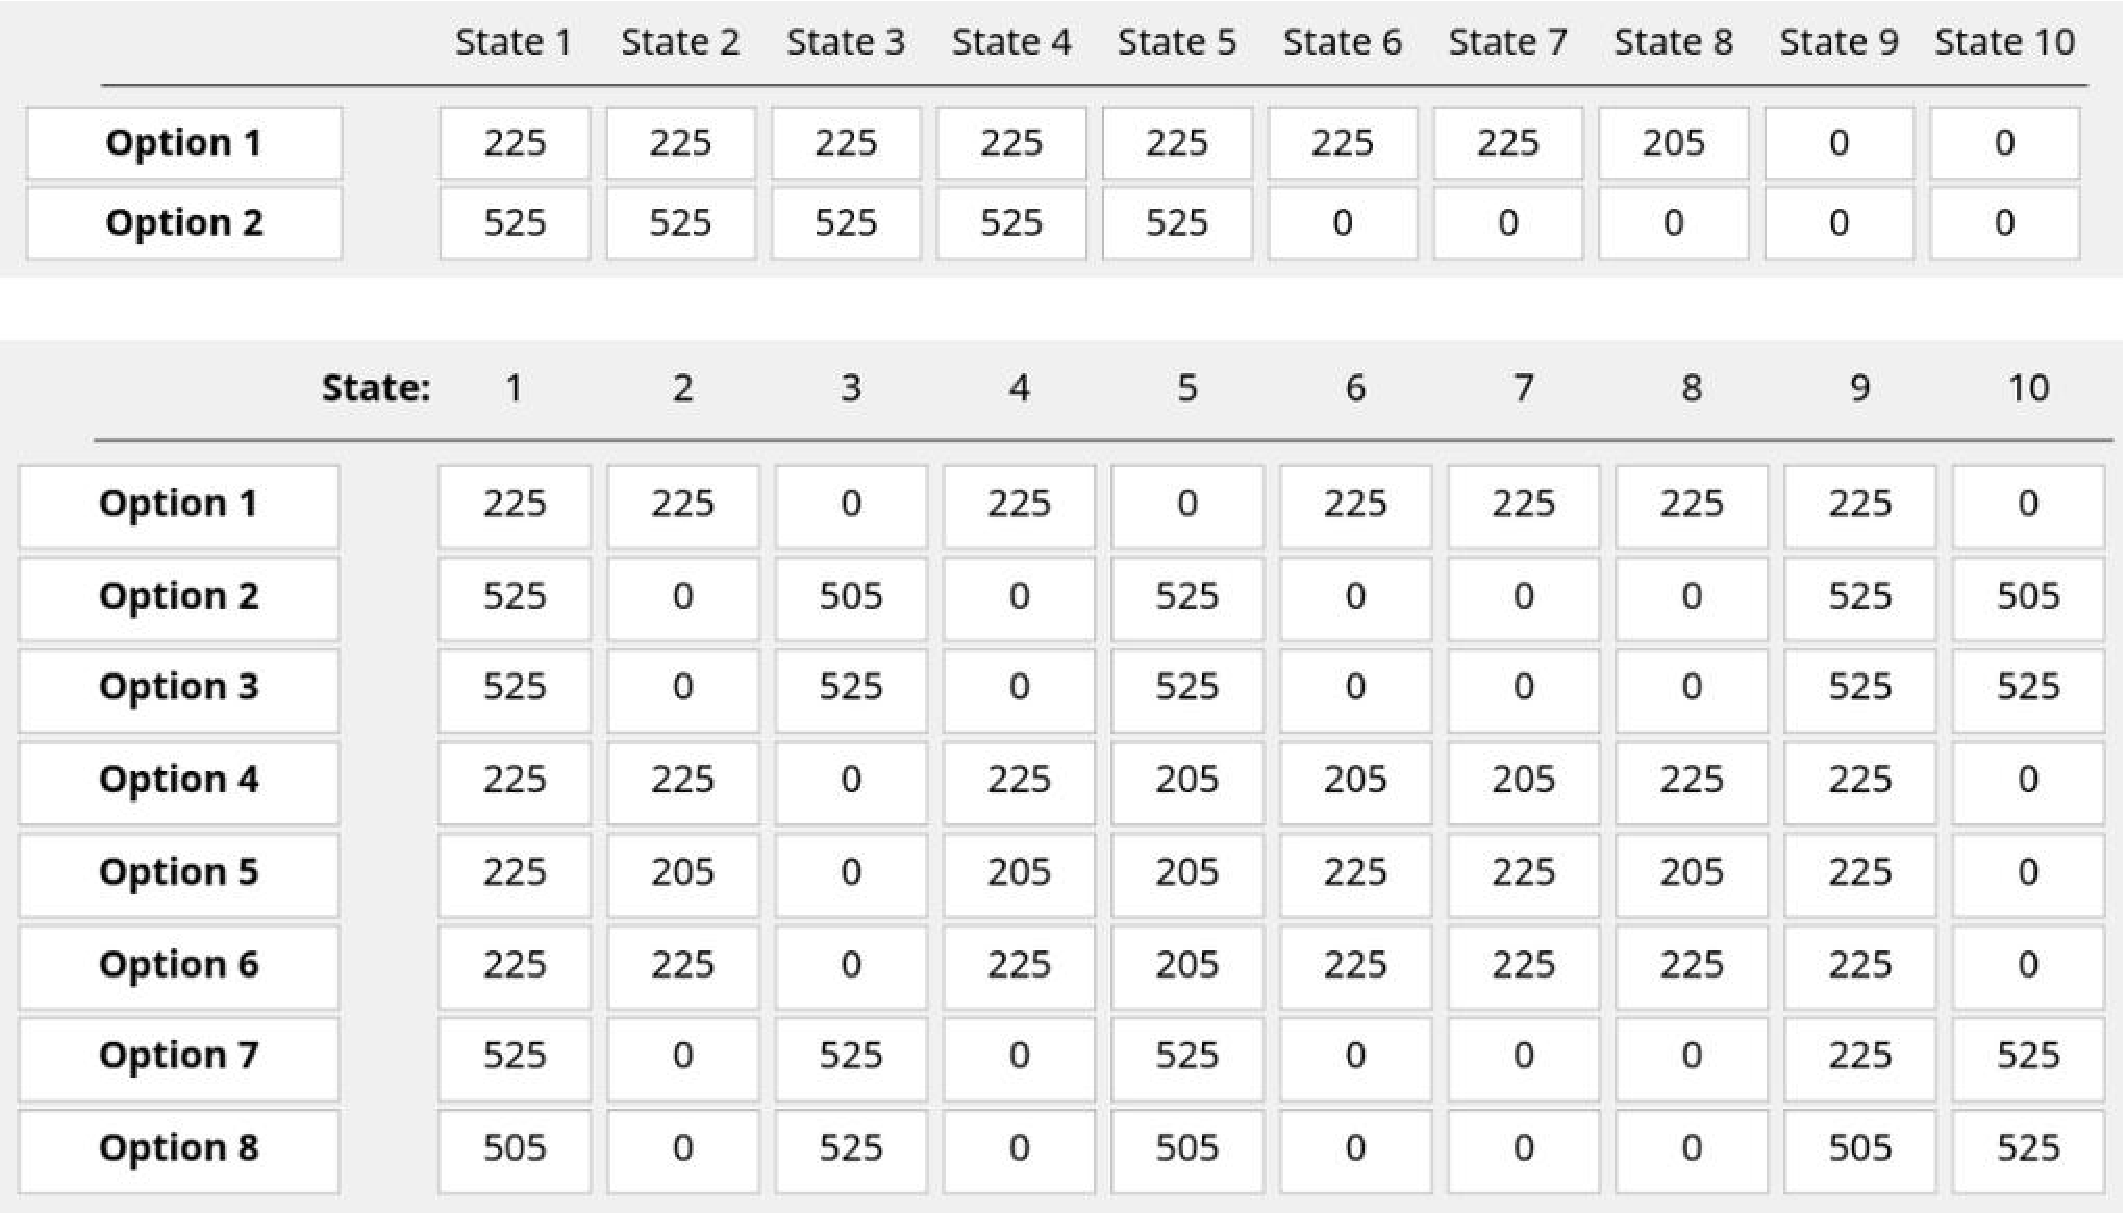
\includegraphics[width = .8\textwidth]{Figure_ExampleScreens.pdf}
\end{figure}
\begin{itemize}
	\item<2-> For further distraction: 4 filler tasks in between
	\item<3-> 8 rounds: 5' pre-view --- 5' algorithm choice---8' decision/waiting time\vspace{-.2cm}
\end{itemize}	
}

 	\frame{\frametitle{Sample, Incentives \& Procedure}
 		\begin{itemize}
 			\item \twi{Recruitment:} Prolific UK, online (z-Tree); preregistered target 120/treatment before exclusions.
 			\item \twi{Exclusions (preregistered):} bot/slider checks, comprehension after 2nd attempt, self-reported AI use, super-fast log-times, incomplete data.
 			\item \twi{Final sample:} \textbf{N = 233} \;(EV: $n=118$,\; Prefs: $n=115$).
 			\item \twi{Incentives:} GBP 2.00 base + one randomly drawn Part-2 round (1 penny / point); up to GBP 8.90 bonus. Mean earning GBP 4.14, median duration $\sim$16 min.
% 			\item \twi{Ethics:} IRB approval by GfeW (cert.\ 19HBJNwQ); informed consent.
 		\end{itemize}
 	}

 	\frame{\frametitle{Preregistered Hypothesis \& Analysis Plan}
 		\begin{itemize}
 			\setlength\itemsep{0.6em}
 			\item \twi{\textbf{H1.}} People are more likely to delegate financial decisions to an \textbf{EV-maximising} algorithm than to a \textbf{personalised} algorithm that incorporates their (revealed) preferences.
 			\item \twi{Primary tests (preregistered):}
 			\begin{itemize}
 				\item[(1)] One-sided \textbf{Boschloo} exact test on \textbf{Round-1} delegation (first contact)
 				\item[(2)] One-sided \textbf{WMW} test on participant-level mean delegation across Part~2
 			\end{itemize}
 			\item \twi{Preregistered LPM:} decision-set FE, participant-clustered SE, treatment\,$\times$%\,
 			\linebreak period interaction, share of prior delegated rounds with zero payoff.
 			\item \twi{Exploratory:} categorical \textit{never-delegation}, win-stay/lose-shift, ex-post reason items.
% 			\item Preregistration: \texttt{\footnotesize https://aspredicted.org/7un5qf.pdf}
 		\end{itemize}
 	}

 	\frame{\frametitle{Main Results: First Contact}
 		\begin{columns}
 			\begin{column}{0.5\textwidth}
 				\begin{itemize}
 					\item \twi{Benchmark:} only $\sim$34--35\% of \textit{self-chosen} options were non-dominated; delegated rounds paid on average \twi{$\sim$25\% more} than self-decided ones $\Rightarrow$ delegation is the instrumentally rational thing to do.
 					\item<2-> \twi{Round 1:} \textcolor{lightblue}{\textbf{66.9\% (EV)}} vs.\ \textcolor{lightblue}{\textbf{55.8\% (Prefs)}}.
 					\item<2-> Boschloo exact test, one-sided: \twi{$p = 0.0413$} $\Rightarrow$ \textbf{H1 supported at first contact.}
 					\item<3-> Treatment gap concentrated in the first decision.
 				\end{itemize}
 			\end{column}
 			\begin{column}{0.5\textwidth}
 				\only<2->{
 				\begin{figure}
 					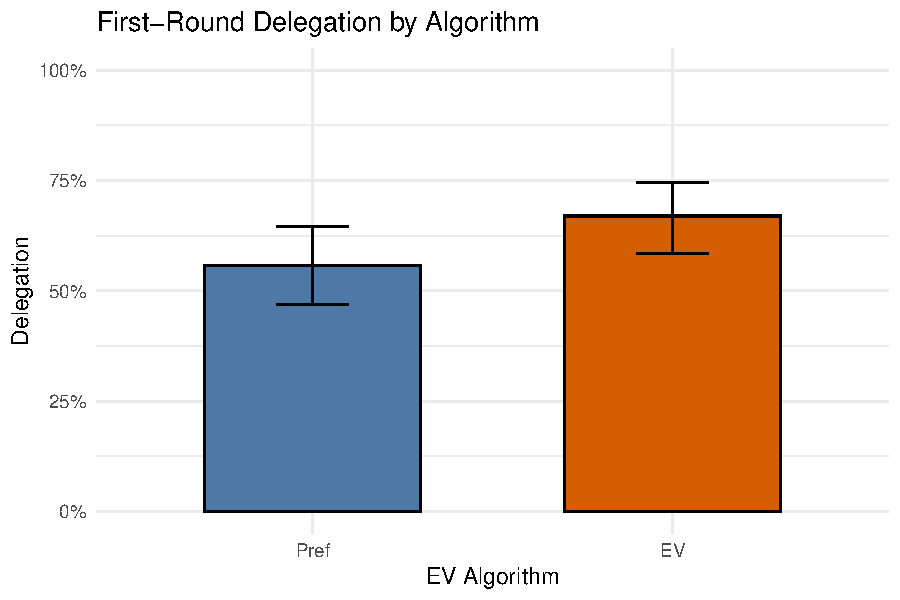
\includegraphics[width=\textwidth]{FirstRdPlot.pdf}
 				\end{figure}}
 			\end{column}
 		\end{columns}
 	}

 	\frame{\frametitle{Main Results: Repeated Decisions}
 		\begin{columns}
 			\begin{column}{0.5\textwidth}
 				\begin{itemize}
 					\item \twi{Average delegation:} no significant treatment difference overall (WMW one-sided $p = 0.2425$).
 					\item Preregistered LPM (decision-set FE, clustered SE):
 					\begin{itemize}
 						\item EV main effect: $\beta = -0.049$, $p = 0.56$
 						\item EV $\times$ period: $\beta = 0.002$, $p = 0.87$
 						\item Share of prior \textit{zero}-payoff delegated rounds: \twi{$\beta = -0.385$, $p < 0.001$}
 					\end{itemize}
 					\item Convergence after Round 1 driven \twi{more by a decline in EV} than by a rise in Prefs.
 					\item But: first-contact decisions can determine whether users \textit{come back at all}.
 				\end{itemize}
 			\end{column}
 			\begin{column}{0.5\textwidth}
 				\begin{figure}
 					
\includegraphics[width=\textwidth]{Figure1_AverageDelegation.pdf}
 				\end{figure}
 			\end{column}
 		\end{columns}
 	}

 	\frame{\frametitle{Categorical Non-Delegation\;\;\small{(not preregistered)}}
 		\begin{columns}
 			\begin{column}{0.5\textwidth}
 				\begin{itemize}
 					\item \twi{Never-delegators:}
 					\begin{itemize}
 						\item \textcolor{lightblue}{\textbf{15.7\%}} in Prefs ($18/115$)
 						\item \textcolor{lightblue}{\textbf{3.4\%}} in EV ($4/118$)
 					\end{itemize}
 					\item Always-delegators show the opposite, weaker pattern (13.6\% Prefs vs.\ 19.1\% EV).
 					\item Never-delegators do \textit{not} differ in age, income, education, gender, time spent, financial risk-taking, AI usage, or reliability.
 					\item Within Prefs: never-delegators report (weakly) \textit{higher} satisfaction with Part-1 choices ($\Rightarrow$ not driven by dislike of the elicited profile).
 					\item \twi{Replication} in earlier (PhD-thesis) study: 32/189 vs.\ 17/187, Boschloo $p = 0.0135$.
 				\end{itemize}
 			\end{column}
 			\begin{column}{0.5\textwidth}
 				\begin{figure}
 					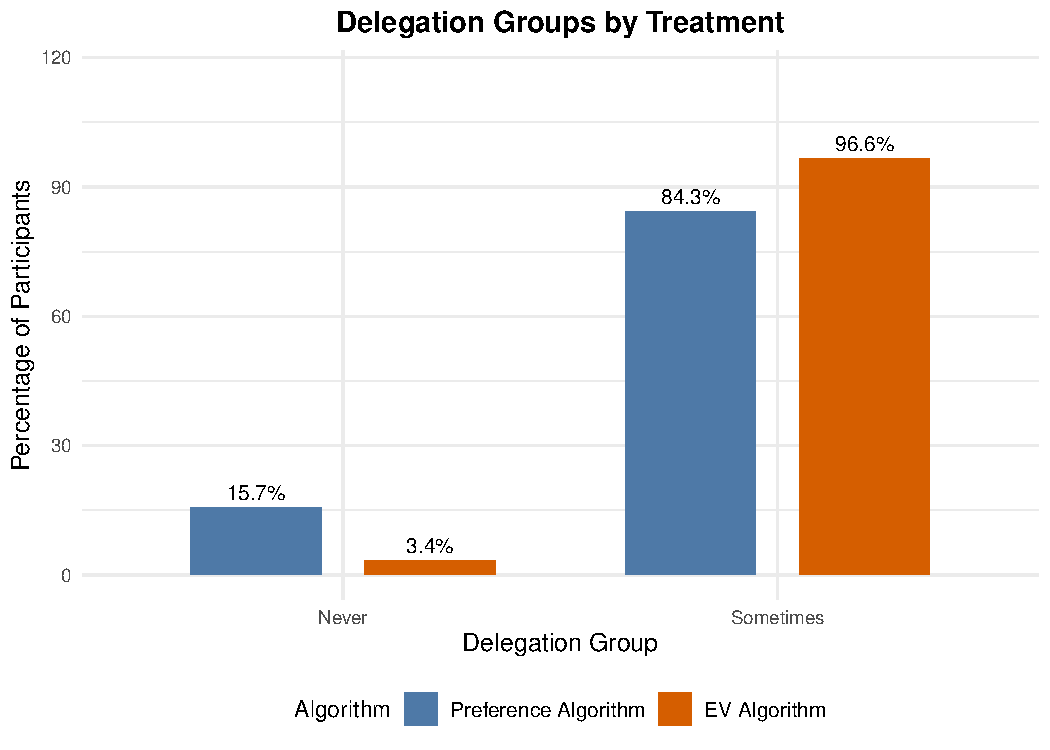
\includegraphics[width=\textwidth]{Figure4_DelegationGroups.pdf}
 				\end{figure}
 			\end{column}
 		\end{columns}
 	}
 	
 	\logo{}

 	\frame{\frametitle{Mechanisms: \textit{What} deters delegation differs by algorithm}
% 		\begin{columns}
% 			\begin{column}{0.55\textwidth}
 				\begin{itemize}
 					\item<2> LPM of individual delegation on \textit{expected non-preferred} and \textit{expected ``completely weird''} choices, $\times$ treatment, controlling for round, Part-1 confidence, risk preferences, task FE:
% 					\item Expected \twi{non-preferred} choices:
% 					\begin{itemize}
% 						\item Prefs: $\beta = -0.058$, $p < 0.001$
% 						\item EV interaction: $+0.035$, $p = 0.09$
% 					\end{itemize}
% 					\item Expected \twi{``completely weird''} choices:
% 					\begin{itemize}
% 						\item Prefs: $\beta = +0.007$, ns
% 						\item EV interaction: $-0.070$, $p = 0.003$
% 					\end{itemize}
% 					\item[\twi{$\triangleright$}] \textit{Non-preferred} deters under \textbf{Prefs}; \textit{extreme errors} deter under \textbf{EV}.
 				\end{itemize}
% 			\end{column}
% 			\begin{column}{0.45\textwidth}
 				\begin{figure}
 					\only<2>{
 						
\includegraphics[width=.75\textwidth]{CoefPlotBadAbsurd.pdf}}
 					\only<1>{
						
\includegraphics[width=.75\textwidth]{ExpectedBadAndAbsurdChoicesByTrmt.pdf}}	
 				\end{figure}
% 			\end{column}
% 		\end{columns}
 	}


%This redefines the background for the regular slides(i.e. the smaller logo in the top-right corner)
\logo{
\includegraphics[scale = 0.25]{logo_twi_cmyk.pdf}\vspace{225pt} \hspace{-.12cm}}


 	\frame{\frametitle{Mechanisms: Self-reported reasons}
 		\begin{itemize}
 			\item Differences run more by \textit{delegator type} than by treatment.
 			\item \twi{Delegators} (vs.\ never-delegators) more often cite performance motives (70.1\% vs.\ 36.4\%: ``computer would choose better'').
 			\item \twi{Never-delegators} more often cite distrust of the algorithm and responsibility for the choice (63.6\% vs.\ 38.9\%).
 			\item Crucially: they want responsibility for the \twi{choice}, \textit{not} for the \twi{outcome} $\Rightarrow$ this is a positive valuation of \textbf{choice authority}, not blame-avoidance.
 			\item Items on being algorithmically analysed and on opacity (``don't know how it chooses'') are rarely selected $\Rightarrow$ not a transparency story.
 			\item[\twi{$\triangleright$}] Consistent with \textit{control / decision-autonomy} as a driver of acceptance (Schaap et al., 2024; Ivanova-Stenzel \& Tolksdorf, 2025).
 		\end{itemize}
 	}

 	\frame{\frametitle{Dynamics: win-stay/lose-shift}%\;\;\small{(secondary)}}
 		\begin{columns}
 			\begin{column}{0.5\textwidth}
 				\begin{figure}
					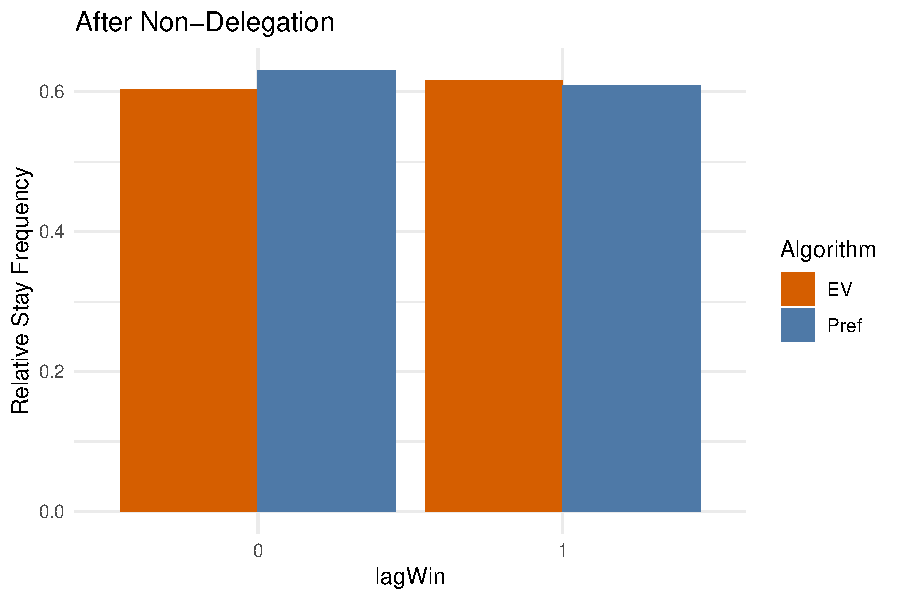
\includegraphics[width=\textwidth]{WinStay_lagNonDeleg.pdf}
				\end{figure}
% 				\begin{itemize}
% 					\item Prefs: prior win $\rightarrow$ slightly \textit{higher} stay probability ($\beta = 0.043$, $p = 0.19$).
% 					\item EV $\times$ prior win: $\beta = -0.102$, $p = 0.041$ $\Rightarrow$ in EV, participants \textit{shift} more after non-zero payoffs than after zeros.
% 					\item Stay rates after losses: 69\% (Prefs) vs.\ 65\% (EV).
% 					\item[\twi{$\triangleright$}] Aggregate dynamics do \textit{not} fit a classic WSLS story; reinforcement appears asymmetric across rules.
% 				\end{itemize}
 			\end{column}
 			\begin{column}{0.5\textwidth}
 				\begin{figure}
 					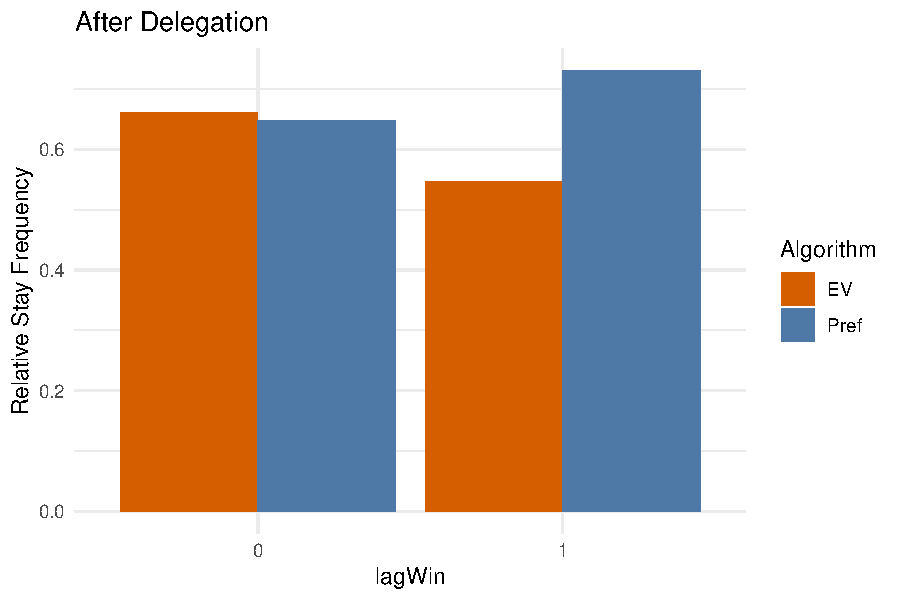
\includegraphics[width=\textwidth]{WinStay_lagDeleg.pdf}
 				\end{figure}
 			\end{column}
 		\end{columns}
 	}

% 	\frame{\frametitle{Limitations}
% 		\begin{itemize}
% 			\item Online experiment with stylised lotteries $\Rightarrow$ external validity to field deployments needs care.
% 			\item Mechanism is \textit{not} causally identified: reason items are ex-post and tied to a hypothetical follow-up question.
% 			\item Short-run repeated interaction only; longer-run adaptation to personalised systems is an open question.
% 			\item Categorical non-delegation is an \textit{exploratory} outcome (preregistered analyses are the Boschloo and WMW tests + the LPM).
% 		\end{itemize}
% 	}

 	\frame{\frametitle{Summary \& Conclusion}
 		\begin{itemize}
 			\setlength\itemsep{0.7em}
 			\item[\twi{1.}] \twi{Preregistered behavioural} comparison of \textit{objective} vs \textit{personalised} decision rules $\Rightarrow$ personalisation does \textit{not} increase delegation.
 			\item[\twi{2.}] The effect is concentrated at \twi{first contact} (Round 1: 66.9\% EV vs 55.8\% Prefs) — and first contact often decides whether users return at all.
 			\item[\twi{3.}] \twi{Categorical non-delegation} is a distinct uptake barrier under personalisation (15.7\% vs 3.4\%), \textit{not} explained by demographics, risk attitudes, AI exposure, or dissatisfaction with the elicited profile.
 		\end{itemize}
% 		\vspace{.4em}
% 		\begin{center}
% 		\textit{\textcolor{lightblue}{The very feature meant to increase subjective fit\\ may encroach on users' sense of choice authority,\\ deterring precisely those who value exercising active control.}}
% 		\end{center}
 	}

 	\frame{\frametitle{Thank you!}
 		\begin{center}
 			\vspace{1cm}
 			\Large \twi{Thank you --- and looking forward to your questions.}\\[1.2cm]
 			\normalsize
 			Irenaeus Wolff $\;\cdot\;$ \texttt{wolff@twi-kreuzlingen.ch}\\[.3cm]
 			Lara Suraci $\;\cdot\;$ DG Cities\\[.6cm]
 			\footnotesize Preregistration: \texttt{https://aspredicted.org/7un5qf.pdf}%\\
% 			Paper, data \& code available upon publication.
 		\end{center}
 	}

\end{document}
